%% Volcanic Sedimentation Rates and Archaeological Visibility in Java
%% JASREP v2.0 — Formatted for Journal of Archaeological Science: Reports (Elsevier)
%% Structural rewrite from EGQSJ v1.0: all lists→prose, language tightened
%% Submission route: subscription (zero APC)

\documentclass[12pt,a4paper]{article}
\usepackage[utf8]{inputenc}
\usepackage[T1]{fontenc}
\usepackage{graphicx}
\usepackage{amsmath}
\usepackage{natbib}
\usepackage{booktabs}
\usepackage{hyperref}
\usepackage[left=2.5cm,right=2.5cm,top=2.5cm,bottom=2.5cm]{geometry}
\usepackage{lineno}
\usepackage{setspace}
\doublespacing
\linenumbers

\begin{document}

\title{Multi-Site Calibration of Volcanic Sedimentation Rates and Implications for Archaeological Visibility in Java, Indonesia}

\author{Mukhlis Amien\textsuperscript{1,*} \and Go Frendi Gunawan\textsuperscript{1}}

\date{}

\maketitle

\noindent\textsuperscript{1}Lab Data Sains, Universitas Bhinneka Nusantara, Malang, Indonesia\\
\textsuperscript{*}Correspondence: amien@ubhinus.ac.id

\begin{abstract}
Java hosts 45 active volcanoes in 129,000~km\textsuperscript{2}. Its early archaeological record is strikingly thin compared to volcanic-free regions of the same archipelago. The standard explanation is developmental: Javanese kingdoms simply came later. The explanation advanced here is geophysical: the evidence is buried.

In 1803, a Dutch colonial administrator named Nicolaus Engelhard documented two enormous stone guardian statues at the ruins of Candi Singosari in East Java---each 370~cm tall, carved from monolithic andesite in 1268~CE---with roughly half their bodies below ground. These statues had not been deliberately interred; rather, Gunung Kelud had erupted approximately twenty times in the intervening 535 years, and the landscape had risen around them at approximately 3.5~mm per year. Structures built of wood, brick, and thatch left no comparable marker above the accumulating sediment.

This paper calibrates what that rate means for the archaeological record as a whole. Using four sites with independently documented construction dates and measured burial depths, spanning two volcanic systems (Kelud and Merapi) and roughly 350~km of Java, we establish a mean sedimentation rate of $4.4 \pm 1.2$~mm/yr. The consistency across sites is the central finding: burial is not a local anomaly but appears to operate at a regional scale across Java's volcanic terrain. At this rate, archaeological remains from the Kanjuruhan period (\textasciitilde760~CE) now lie at 4.0--7.8~m depth in the Malang basin---beyond the reach of surface survey and at the upper limit of ground-penetrating radar. Indonesia's oldest conventionally recognized kingdom, Kutai (\textasciitilde400~CE), was found near the present ground surface in volcanic-free Kalimantan; at Javanese sedimentation rates, equivalent remains would lie beneath 7--10~m of volcanic overburden. Spatial analysis of 666 East Java sites confirms the pattern: the observable record maps survey effort and monument durability, not historical settlement intensity. We identify priority zones where high terrain suitability coincides with deep predicted burial, providing a targeting framework for future subsurface investigation.

\medskip
\noindent\textbf{Keywords:} volcanic taphonomy; sedimentation rates; archaeological visibility; East Java; multi-site calibration; survey bias
\end{abstract}


\section{Introduction}

In 1803, a Dutch colonial administrator named Nicolaus Engelhard encountered something at the ruins of Candi Singosari that has not received the theoretical attention it deserves. Two enormous stone guardian statues---\textit{Dwarapala}, each 370~cm tall and carved from a single block of andesite---stood with roughly half their bodies below the ground. They had been installed in 1268~CE, during the reign of King Kertanegara of the Singosari kingdom \citep{kinney2003}. The ground had risen around them at approximately 3.5~mm per year, driven by 535 years of repeated eruptions from Gunung Kelud, 35~km to the east. Only their scale made them visible at all.

Hindu-Buddhist kingdoms flourished on Java from at least the 4th century~CE, yet the material record of early Javanese polities is strikingly sparse compared to contemporaneous societies elsewhere in Southeast Asia. The kingdom of Kutai Martadipura in Kalimantan---conventionally regarded as Indonesia's oldest polity (\textasciitilde400~CE)---is known from inscribed stone pillars found near the modern ground surface in a region with zero active volcanoes \citep{vogel1918,coedes1968}. The argument of this paper is direct: the oldest Indonesian kingdom is the most \textit{visible} one. At the sedimentation rate established here, a Javanese inscription of the same age as Kutai's Yupa pillars now lies beneath approximately 7~m of volcanic overburden---invisible to surface survey, beyond the reach of conventional ground-penetrating radar. The apparent chronological primacy of non-volcanic Kalimantan over volcanic Java reflects differential preservation, not differential history.

The mechanism at work is not the catastrophic burial familiar from Pompeii, Akrotiri, or Cer\'{e}n---single eruptions sealing settlements in hours \citep{sigurdsson1985,doumas1983,sheets1992}. It is \textit{cumulative} sedimentation: repeated small eruptions depositing millimeters per event, accumulating to meters over centuries (Sect.~2.3). In Java, every point on the island lies within approximately 27~km of an active vent \citep{vanbemmelen1949}, placing the entire landmass within the depositional range of at least one volcanic center. The Dwarapala statues provide direct photographic documentation of this process at a known, measurable rate (Fig.~\ref{fig:dwarapala_photos}).

\begin{figure*}[t]
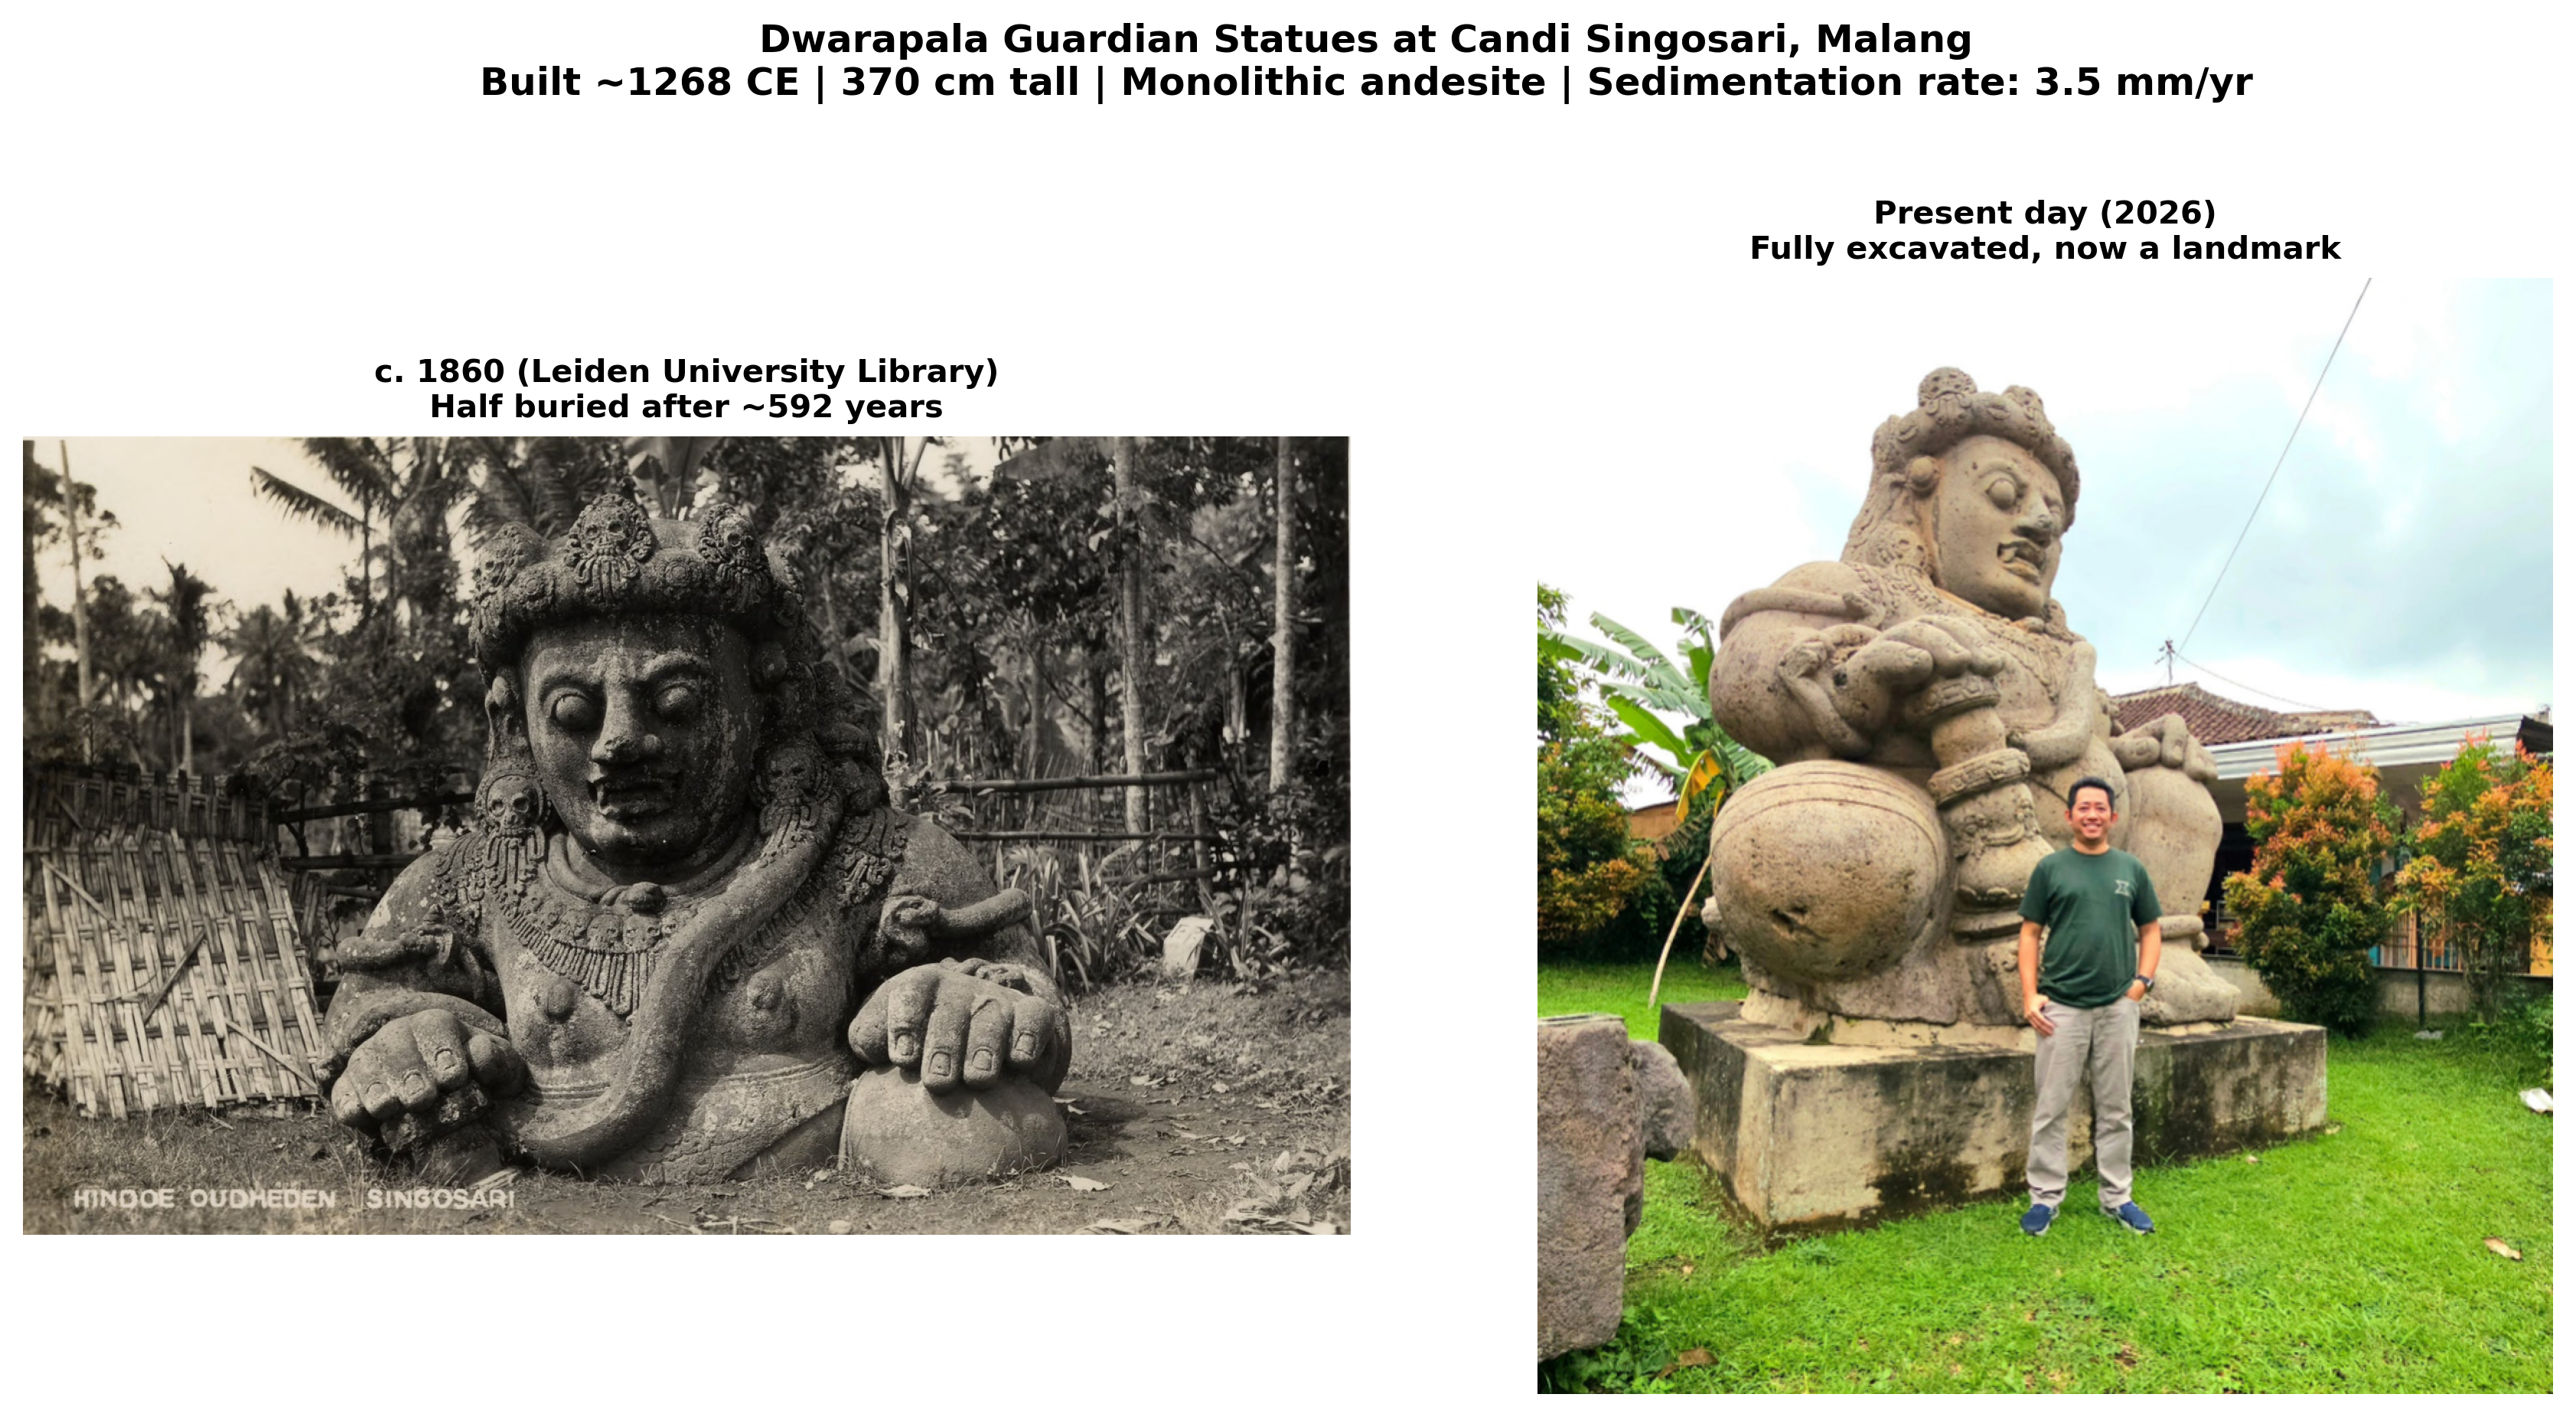
\includegraphics[width=12cm]{figures/fig0_dwarapala_comparison.png}
\caption{Dwarapala guardian statues at Candi Singosari, Malang, East Java. Left: colonial-era photograph (c.~1860) from the Leiden University Library archives, showing the statue partially buried beneath volcanic sediment---only the head, shoulders, and hands remain visible above the accumulated overburden. Right: present-day condition after excavation, revealing the full 370~cm height. The statues were constructed \textasciitilde1268~CE during the reign of Kertanegara; approximately 185~cm of volcanic overburden accumulated by their rediscovery in 1803~CE, yielding a calibrated sedimentation rate of 3.5~mm/yr (Sect.~3.2).}
\label{fig:dwarapala_photos}
\end{figure*}

Surface visibility is a recognized problem in archaeological survey \citep{wandsnider1992,french2003}, but its implications for volcanic landscapes in island Southeast Asia have been largely unexplored. Research in the region has focused on monumental stone architecture---the class of evidence most resistant to burial \citep{degroot2009}---producing an inherent circularity: stone temples are found because they protrude through sediment; their distribution is interpreted as reflecting settlement patterns; and the wooden settlements that constituted the overwhelming majority of historical habitation are overlooked entirely.

The empirical foundation of this study is a four-site calibration. We compiled construction dates and measured burial depths for four archaeological sites: the Dwarapala statues at Candi Singosari (\textasciitilde1268~CE, Kelud volcanic system) and three Hindu-Buddhist temples near Merapi in Central Java (Sambisari, Kedulan, and Kimpulan, all 9th century~CE). These span roughly 350~km of Java and two geologically distinct volcanic systems. Kelud has produced 37 confirmed eruptions since 1000~CE \citep{gvp2024}. Merapi is one of the world's most persistently active stratovolcanoes \citep{gertisser2012}. The sedimentation rates converge within a factor of two---a finding that was not guaranteed and that we consider central to the argument.

Those rates are applied to project burial depths for successive historical periods: Kanjuruhan-era (\textasciitilde760~CE) remains in the Malang basin are predicted to lie at 4.0--7.8~m---exceeding the reach of surface survey and approaching the upper limit of ground-penetrating radar \citep{putra2019}. A spatial analysis of 666 known archaeological sites in East Java tests the corollary: if the taphonomic argument is correct, the observable record should map survey effort and monument scale, not settlement patterns. Priority zones for future subsurface investigation are identified where terrain suitability and predicted burial depth are both high.


\section{Background}

\subsection{Java as a volcanic burial zone}

Java hosts 45 active volcanoes across approximately 129,000~km\textsuperscript{2}---a volcanic density of 0.35 per 1,000~km\textsuperscript{2}, the highest of any major Indonesian island and approximately six times that of Sumatra (0.06/1,000~km\textsuperscript{2}) \citep{vanbemmelen1949}. The average spacing between volcanic centers is approximately 54~km, meaning that no point on Java lies more than approximately 27~km from the nearest active volcano. Since tephra from VEI~3--4 eruptions can deposit measurable ash at 50--100+~km from the source \citep{newhall1982}, the entire island falls within the depositional range of at least one---and typically multiple---volcanic centers. The relevant archaeological question is therefore not whether volcanic sedimentation occurs at a given location, but how much has accumulated since a site was occupied---a function of distance from active vents, local topography, and eruption history.

East Java province alone encompasses seven major active centers: Kelud, Semeru, Arjuno-Welirang, Bromo, Lamongan, Raung, and Ijen. The Brantas River basin---which hosted the Singosari (1222--1293~CE) and Majapahit (1293--\textasciitilde1500~CE) kingdoms---sits in the depositional path of Kelud (35~km east), Arjuno-Welirang (25~km north), and Semeru (60~km southeast). Kelud alone has produced 37 confirmed eruptions since 1000~CE \citep{gvp2024,maeno2019}.

In Central Java, Mount Merapi---one of the world's most active stratovolcanoes---has buried a cluster of 9th-century Hindu-Buddhist temples to depths of 3--7~m \citep{lavigne2000,thouret2000}. These buried temples (Sambisari, Kedulan, Kimpulan) were discovered accidentally during modern construction and mining activities, not through systematic archaeological survey.

\subsection{The observable archaeological record in East Java}

Our compilation of known archaeological sites in East Java (Sect.~3.1) identified 666 unique entries, of which only 391 (59\%) have usable spatial coordinates. The dataset is dominated by stone monuments (\textit{candi}) from the Singosari and Majapahit periods (13th--15th centuries~CE) \citep{kinney2003}. Earlier periods are poorly represented: pre-10th century sites constitute less than 5\% of the geocoded total.

This temporal distribution reflects two complementary pressures. Survey has historically concentrated on the Singosari-Majapahit heartland around Blitar, Malang, and Mojokerto. Simultaneously, older sites have accumulated more volcanic overburden and are therefore less likely to be exposed at the modern ground surface.

A conceivable objection is that this pre-10th century absence reflects genuine demographic scarcity rather than taphonomic loss. This objection fails quantitatively. Three independent estimation approaches yield convergent population estimates for pre-400~CE Java. First, ethnographic carrying capacity estimates for tropical island Southeast Asian agriculture range from approximately 5 to 30 persons/km\textsuperscript{2} for swidden and early wet-rice systems \citep{bellwood2017,kirch2000,baylisssmith1980}; applied to Java's habitable lowlands (approximately 65,000~km\textsuperscript{2}, based on terrain suitability thresholds), these densities yield approximately 325,000 to 1,950,000 inhabitants. Second, demographic back-projection from early-modern anchors (roughly 4.0 to 5.0 million on Java by 1600~CE; \citealp{reid1988}) using plausible Malthusian growth rates implies a pre-400~CE baseline of similar order to the carrying-capacity result. Third, comparison with contemporaneous Austronesian polities---Dvaravati Thailand (300,000--500,000), the Philippines (200,000--500,000), early Sriwijaya (50,000--150,000)---places Java at or above the regional median. The three approaches converge on a central estimate of approximately 1 to 2 million inhabitants at 400~CE, with a conservative lower bound near 600,000. At standard Austronesian village sizes of 100 to 200 persons, this range implies between 3,000 and 20,000 settlements of standard archaeological visibility. The observed count of pre-400~CE sites in the volcanic interior is 0 to 3, representing a gap of between approximately 1,000-fold and 7,000-fold depending on the population estimate used. Low population density alone cannot account for a discrepancy of this magnitude.

The inscription record provides independent confirmation. Systematic reading of all 268 surviving Javanese inscriptions in the DHARMA epigraphic database (8th--13th centuries~CE) \citep{dharma2024} reveals that 170 (63.4\%) explicitly mention organic building materials---wood (\textit{kayu}), bamboo (\textit{bambu}), palm thatch (\textit{atap}), palm fiber (\textit{ijuk})---while only 73 (27.2\%) mention stone or brick (binomial $p < 0.0001$). The people who carved these stone inscriptions lived predominantly in structures that do not survive in the archaeological record. The archaeological blank of volcanic Java reflects a preservation filter that passes stone and rejects wood, not an absence of habitation.

\subsection{Volcanic taphonomy}

The volcanological literature on archaeological burial is dominated by catastrophic events: Pompeii sealed in eighteen hours, Candi Sambisari buried over roughly a thousand years. These are fundamentally different processes that produce different archaeological signatures.

Catastrophic volcanic burial---a single eruption sealing an entire settlement in hours---is well documented \citep{sigurdsson1985,doumas1983,sheets1992} and, precisely because it is dramatic, attracts sustained excavation attention. \textit{Cumulative} volcanic burial, by contrast, generates no single event to excavate. Ash arrives in centimeters per eruption, lahars rework it downslope, and every decade the ground surface is fractionally higher than the decade before. After five centuries, a surface that was once at ground level lies two meters underground. After fifteen centuries, it may lie at six meters depth. No emergency response is triggered; no excavation follows. The site becomes, gradually and completely, invisible to surface survey.

\subsection{The Kutai comparison}

The oldest known kingdom in the Indonesian archipelago is Kutai Martadipura (\textasciitilde400~CE), located in East Kalimantan---a region with zero active volcanoes across 544,000~km\textsuperscript{2} \citep{vogel1918}. Its Yupa inscriptions were found near the present ground surface.

The contrast with Java is stark: Java has 45 active volcanoes in 129,000~km\textsuperscript{2}; Kalimantan has none in 544,000~km\textsuperscript{2}. At the mean Javanese sedimentation rate of 4.4~mm/yr, a Kutai-era (\textasciitilde400~CE) inscription in the Malang basin would now lie beneath 4--10~m of volcanic overburden---invisible to any surface survey. The same inscription in Kalimantan sits exactly where it was placed 1,600 years ago, because there is no volcanic sedimentation to bury it.

Kutai's apparent chronological primacy over Javanese polities of similar or greater antiquity may therefore reflect differential preservation conditions rather than genuine temporal precedence \citep{coedes1968,miksic2004}. The ``oldest kingdom'' is the most \textit{visible} one---a direct consequence of the volcanic density asymmetry between islands.

\subsection{The West Java control: within-island preservation asymmetry}

A cross-island comparison between Java and Kalimantan, while suggestive, is subject to the objection that the two islands differ in many respects besides volcanism: ecology, trade routes, cultural trajectories, and research history. The strongest evidence for taphonomic bias comes not from a cross-island comparison but from a within-island one.

West Java's non-volcanic coastal zone preserves a rich pre-400~CE material record that the volcanic interior entirely lacks---on the same island, during the same broad period. The Buni Cultural Complex (Tangerang coast, \textasciitilde200~BCE--500~CE) represents a dense concentration of organic-rich cultural material---pottery, glass and carnelian beads, iron tools, bronze ornaments---distributed across dozens of sites in a region of zero active volcanism \citep{wibisono1994,bellina2014}. Batujaya (Karawang regency, 2nd--5th century~CE), on the same non-volcanic coastal plain, preserves a substantial brick Buddhist complex---the oldest confirmed Buddhist architectural remains in the archipelago \citep{manguin2011}. Both complexes document demographically significant, organizationally complex societies in Java during precisely the period for which the volcanic interior offers nothing.

This within-island asymmetry is consistent with the predictions of the taphonomic framework: same island, same broad time window, with the critical difference being geology---non-volcanic coastal plain versus volcanic alluvial basin. A caveat is necessary: the Buni and Batujaya communities were embedded in maritime trade networks connecting the Malay Peninsula and the Indian Ocean \citep{bellina2014,manguin2011}; interior volcanic Java may have supported culturally distinct populations whose material absence reflects genuine difference rather than taphonomic loss. The comparison controls for island-level factors---climate, deep linguistic history, broad ecology---but not for the coastal-interior economic divergence that characterizes much of Island Southeast Asian prehistory. We present it as suggestive evidence, not definitive proof.


\section{Data and Methods}

\subsection{Archaeological site dataset}

We compiled a database of known archaeological sites in East Java province from three complementary sources. First, we queried the OpenStreetMap Overpass API for all features tagged with \texttt{historic=*} within the Jawa Timur administrative boundary (bounding box: 6.5--9.0\textdegree{}S, 111.0--115.0\textdegree{}E), yielding 281 geolocated features. Second, we queried the Wikidata SPARQL endpoint for entities with coordinate property P625 within the same bounding box, recovering 16 precisely located sites. Third, we scraped the Indonesian-language Wikipedia article ``Daftar candi di Indonesia'' for 369 additional entries.

To increase spatial coverage, we geocoded the 369 coordinate-less entries using the OpenStreetMap Nominatim API with progressive query refinement. Of 369 queries, 94 returned valid coordinates within the study area (25.5\% success rate). After spatial deduplication within a 100~m radius, the final dataset contains 666 unique site entries, of which 391 have usable coordinates (58.7\% geocoding rate). Within the East Java analytical bounds, 383 geocoded sites were used for spatial analysis.

It should be noted that this dataset is heavily biased toward stone monuments (\textit{candi}) that survived volcanic burial due to their monumental scale. Wooden settlements, which likely constituted the vast majority of historical habitation, are systematically absent---precisely the pattern predicted by the taphonomic bias hypothesis.

\subsection{The Dwarapala calibration}

The primary empirical anchor for the burial depth framework is the pair of Dwarapala guardian statues at Candi Singosari, Malang Regency, East Java. The statues were constructed approximately 1268~CE during the reign of Kertanegara of the Singosari Kingdom and discovered in 1803~CE by the Dutch colonial administrator Nicolaus Engelhard. Each statue stands 370~cm in seated height and weighs approximately 40 tonnes, carved from monolithic andesite. At the time of discovery, approximately half of each statue's body was below the ground surface (``\textit{separuh tubuh terpendam}''), corresponding to an estimated burial depth of approximately 185~cm accumulated over 535 years (1803 $-$ 1268 = 535 years). The resulting sedimentation rate is:

\begin{equation}
  R = \frac{185~\text{cm}}{535~\text{yr}} = 0.35~\text{cm/yr} = 3.5~\text{mm/yr}
\end{equation}

This rate is internally consistent with the documented eruption history of Gunung Kelud. The volcano erupted approximately 20 times between 1268 and 1803~CE, and documented VEI~3--4 eruptions deposit 2--20~cm of ash at the distance of Malang (\textasciitilde35~km from the vent). Twenty eruptions at an average of approximately 5~cm per event would account for approximately 100~cm of the 185~cm total burial. The remainder (\textasciitilde85~cm) is attributable to secondary remobilization (lahars, reworked tephra), contributions from the Semeru and Arjuno-Welirang volcanic systems, and non-volcanic aggradation \citep{gvp2024,maeno2019}. The rates reported here represent \textit{total landscape aggradation} in volcanic terrain, not pure primary tephra accumulation; for archaeological burial, however, the total aggradation rate is the operationally relevant metric regardless of depositional source.

The Dwarapala burial timeline from construction to present is illustrated in Fig.~\ref{fig:timeline}.

\begin{figure}[t]
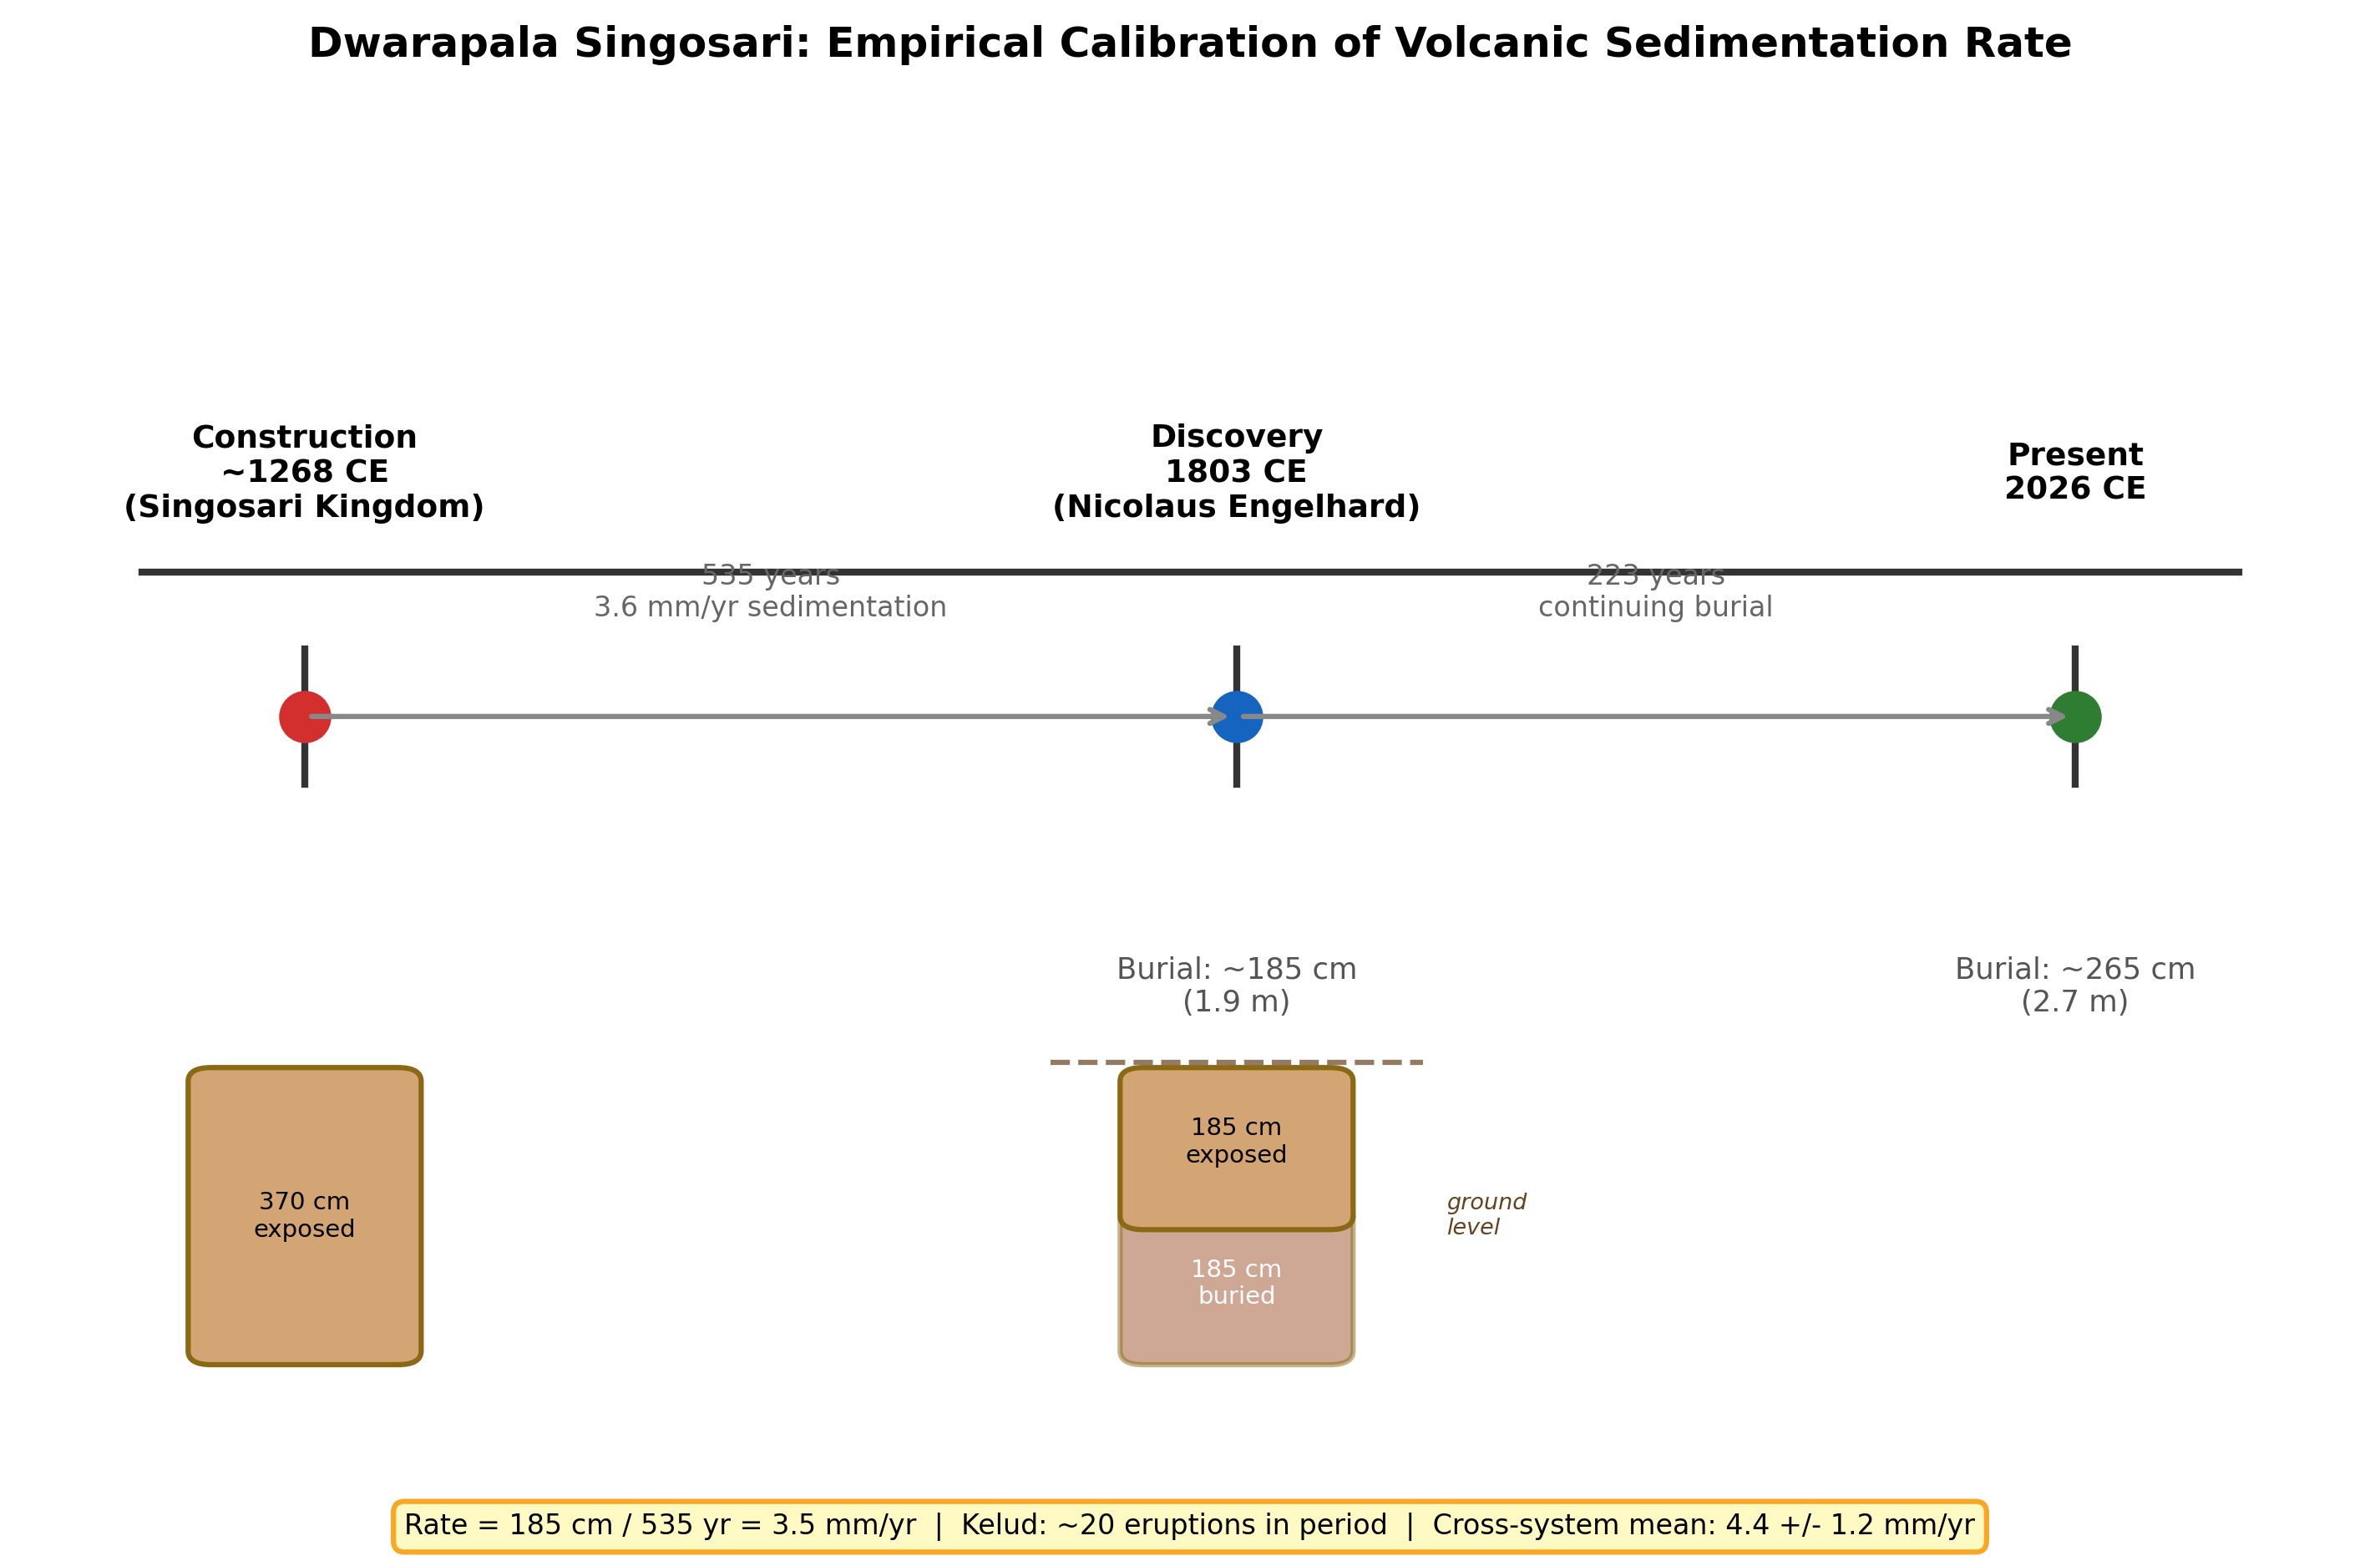
\includegraphics[width=8.3cm]{figures/fig1_dwarapala_timeline.png}
\caption{Dwarapala Singosari burial timeline. The statues were constructed \textasciitilde1268~CE at full height (370~cm) and discovered in 1803~CE with approximately half (185~cm) buried by volcanic sedimentation, yielding a cumulative rate of 3.5~mm/yr. The cross-system mean from four calibration points is $4.4 \pm 1.2$~mm/yr.}
\label{fig:timeline}
\end{figure}

\subsection{Secondary calibration points}

To assess whether the Dwarapala rate is a local anomaly or representative of a Java-wide phenomenon, we compiled three additional calibration points from Central Java's Merapi volcanic system (Table~\ref{tab:calibration}).

\begin{table}[t]
\caption{Empirical calibration points for volcanic sedimentation rates at archaeological sites in Java. BPCB-Jatim and BPCB-DIY are Indonesia's regional heritage conservation agencies (\textit{Balai Pelestarian Cagar Budaya}, Ministry of Education and Culture); burial depths are from their published excavation reports. Sambisari and Kedulan depths are cited in \citet{lavigne2000} and \citet{thouret2000}.}
\label{tab:calibration}
\begin{tabular}{lcccccc}
\toprule
Site & Built (CE) & Discovered & Depth (cm) & System & Rate (mm/yr) & Source \\
\midrule
Dwarapala Singosari & \textasciitilde1268 & 1803 & \textasciitilde185 & Kelud & 3.5 & BPCB Jatim \\
Candi Sambisari & \textasciitilde835 & 1966 & 500--650 & Merapi & 4.4--5.7 & BPCB DIY \\
Candi Kedulan & \textasciitilde869 & 1993 & 600--700 & Merapi & 5.3--6.2 & BPCB DIY \\
Candi Kimpulan & \textasciitilde900 & 2009 & 270--500 & Merapi & 2.4--4.5 & \citet{putra2019} \\
\bottomrule
\end{tabular}
\end{table}

Across all four sites, the computed rates span 2.4--6.2~mm/yr. Taking the midpoint of each site's range (Dwarapala: 3.5; Sambisari: 5.1; Kedulan: 5.8; Kimpulan: 3.5~mm/yr) yields a mean of $4.4 \pm 1.2$~mm/yr (1$\sigma$, $n=4$). The full observed range of 2.4--6.2~mm/yr is used for all subsequent projections. The consistency across two independent volcanic systems---Kelud in East Java and Merapi in Central Java---demonstrates that mm/yr-scale burial of archaeological sites is systematic and Java-wide, not a local anomaly (Fig.~\ref{fig:rates}).

\subsection{Independent validation: eruption--site correlation dataset}

As an independent check on these calibration rates, we compiled a dataset of 51 documented eruption--archaeological site correlations from across 12 volcanic systems in Island Southeast Asia. Sources were historical and colonial-era records documenting specific volcanic events and their effects on specific known sites; 86\% of the evidence was primary (directly observed and recorded, not inferred from proximity). Of the 51 pairs, 24 include physically measured burial depths. The mean measured depth across these 24 sites is 3.41~m (median 2.50~m), consistent with the four-site calibration mean of 4.4~mm/yr applied over a 760-year horizon (expected depth: 3.3~m). This dataset shares no sites with the primary calibration and provides independent confirmation that meter-scale burial is a normal outcome of multi-century volcanic sedimentation at archaeological sites across the region.

\begin{figure}[t]
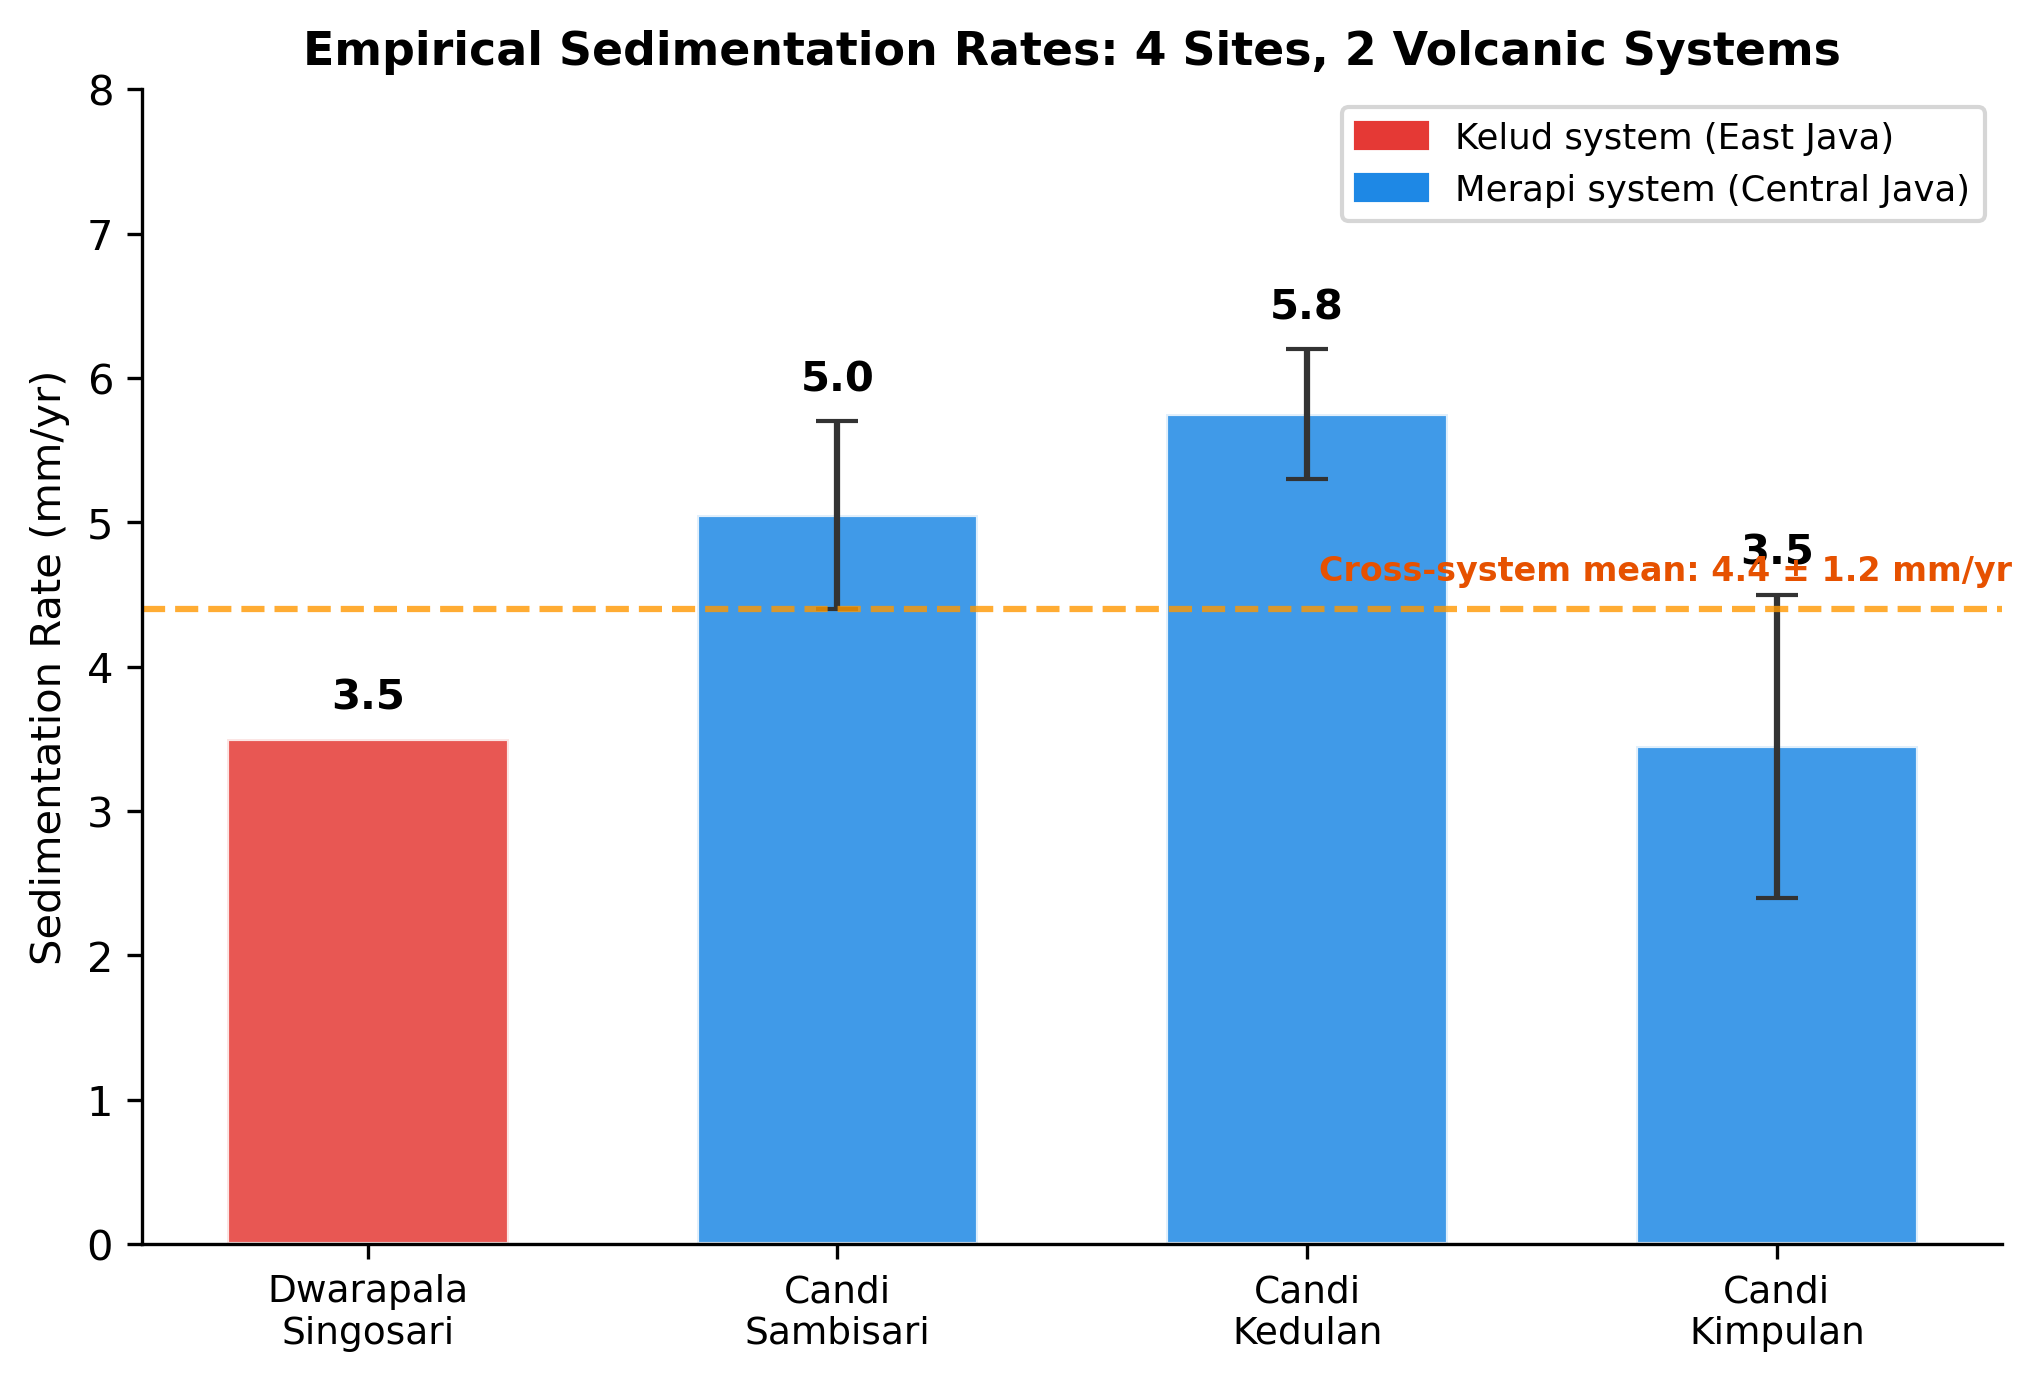
\includegraphics[width=8.3cm]{figures/fig3_calibration_rates.png}
\caption{Empirical sedimentation rates from four archaeological sites across two volcanic systems. Error bars show the range from reported depth uncertainty. The cross-system mean is $4.4 \pm 1.2$~mm/yr.}
\label{fig:rates}
\end{figure}

\subsection{Burial depth projection model}

Using the empirically derived rate range, we estimate expected overburden depth by era according to the linear model:

\begin{equation}
  D(\text{era}) = R \times (T_{\text{present}} - T_{\text{era}})
\end{equation}

\noindent where $R$ ranges from 2.4 to 6.2~mm/yr and $T_{\text{present}} = 2026$~CE. This linear model is a first-order approximation; actual deposition is episodic, with eruption clusters interspersed by quiescent periods and subject to compaction. The wide rate range (2.4--6.2~mm/yr) partially captures this variability. Results are presented in Fig.~\ref{fig:depth}.

\begin{figure*}[t]
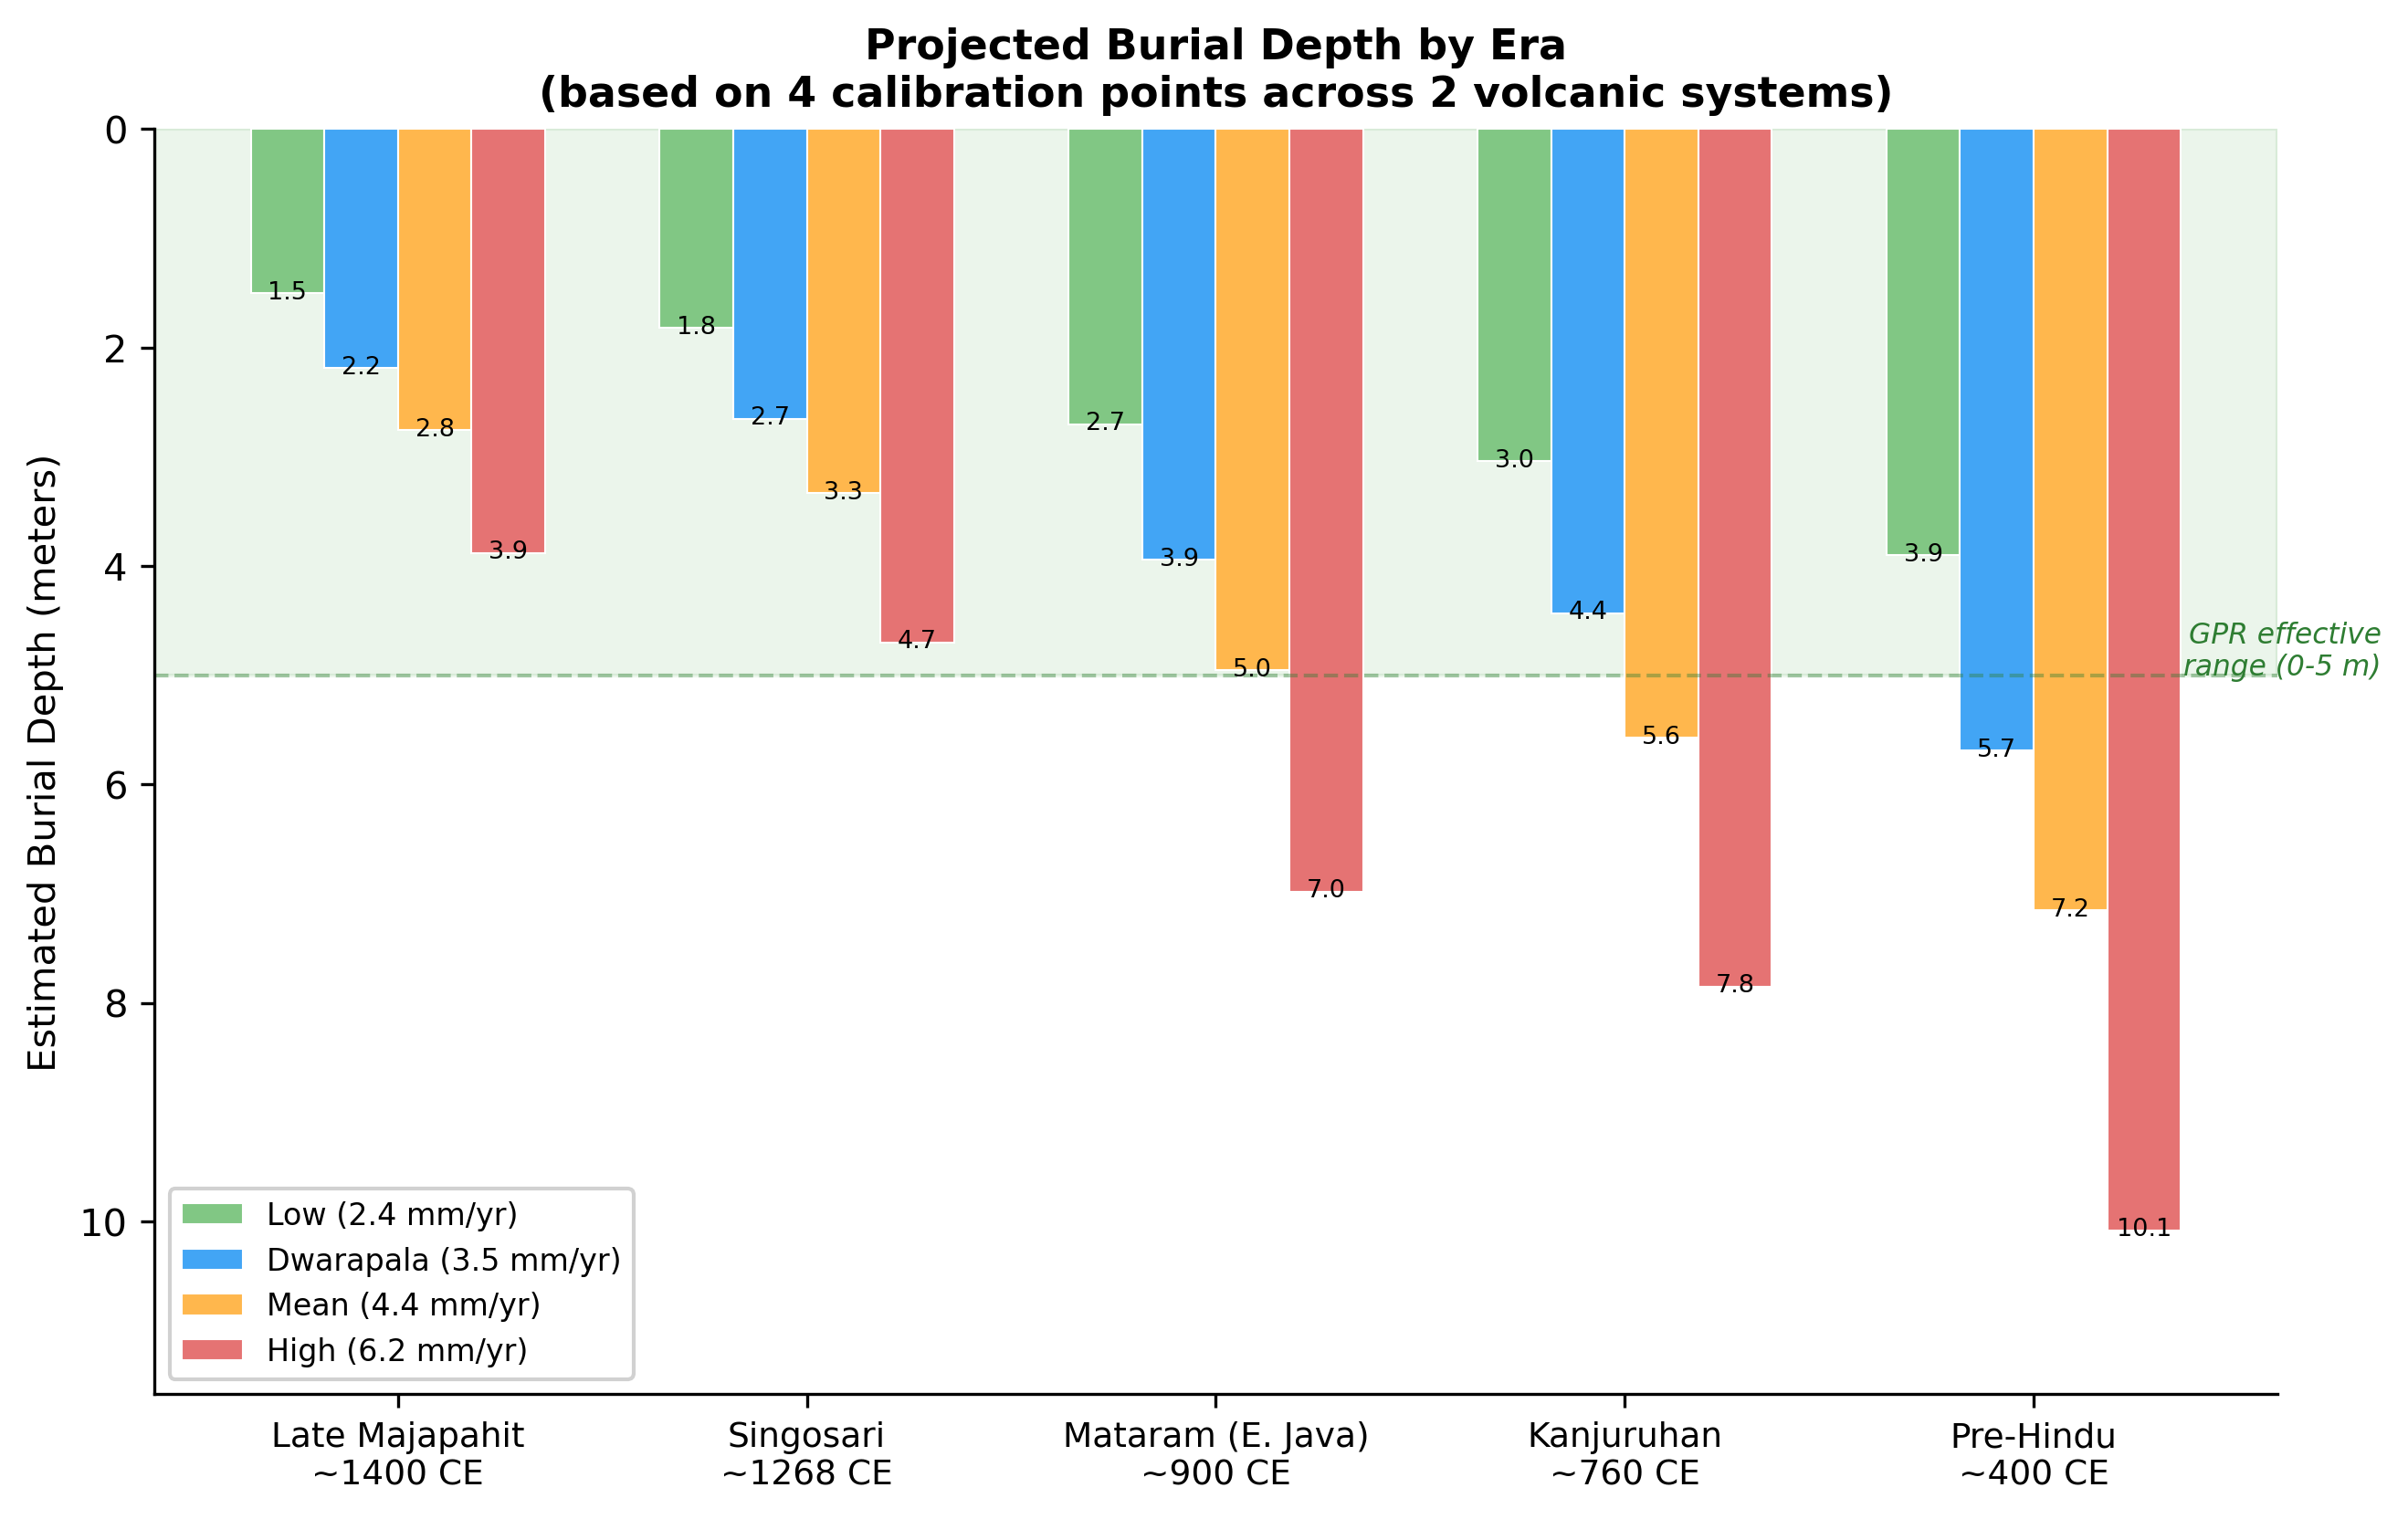
\includegraphics[width=12cm]{figures/fig2_burial_depth_projections.png}
\caption{Projected burial depth by historical era using four empirically-derived sedimentation rates. The green band indicates the effective range of ground-penetrating radar in volcanic sediment (0--5~m). Kanjuruhan-era and earlier remains may exceed GPR detection limits.}
\label{fig:depth}
\end{figure*}

\subsection{Spatial analysis methods}

Two complementary spatial analyses were conducted to examine the relationship between site distribution and volcanic proximity.

In the first analysis, we computed the minimum great-circle distance from each geocoded site to the nearest of seven reference volcanoes. Sites were binned into seven distance bands (0--25, 25--50, 50--75, 75--100, 100--150, 150--200, and 200+~km), and site density was expressed as sites per 1,000~km\textsuperscript{2}. Spearman's rank correlation between distance band midpoint and site density was used to test whether sites are found preferentially near or far from volcanoes.

In the second analysis, we controlled for the effect of terrain suitability on site distribution by constructing a terrain suitability index combining four DEM-derived features: slope, elevation, topographic wetness index (TWI), and a river proximity proxy. The study area was divided into a 25~km $\times$ 25~km grid (187 cells). For each cell, we computed the residual between observed and terrain-predicted site count. Spearman correlation between residual density and distance to the nearest volcano tests the taphonomic bias hypothesis after controlling for terrain preference.


\section{Results}

\subsection{The Dwarapala calibration}

The Dwarapala sedimentation calculation yields a rate of 3.5~mm/year (Sect.~3.2). This rate is internally consistent with documented Kelud eruption histories, which account for approximately 100 of the 185~cm total burial through direct tephra deposition alone. The remaining 85~cm is attributable to secondary remobilization and contributions from other volcanic systems.

The secondary calibration points yield rates of 2.4--6.2~mm/yr across the Merapi system, consistently higher than the Dwarapala rate (3.5~mm/yr) from the Kelud system. This difference is physically plausible: Merapi erupts more frequently than Kelud, and the Central Java sites are closer to their volcanic source. The cross-system mean of $4.4 \pm 1.2$~mm/yr establishes that ongoing volcanic burial is a Java-wide phenomenon with quantifiable, consistent rates.

\subsection{Independent validation}

The 51-pair eruption--site correlation dataset provides a check independent of the four primary calibration sites. Of the 51 pairs, 24 include physically measured burial depths, with a mean of 3.41~m (median 2.50~m). Applying the mean calibration rate of 4.4~mm/yr over 760 years (the midpoint historical horizon) predicts 3.3~m. The independent dataset and the calibration model agree within 3\%. This is consistent with---though not proof of---the calibration rates representing a true regional baseline rather than a monument-specific artefact.

\subsection{Burial depth projections}

Table~\ref{tab:depth} presents key burial depth projections for the Malang basin using the full empirically derived rate range.

\begin{table}[t]
\caption{Projected burial depth by era using empirically-derived sedimentation rates.}
\label{tab:depth}
\begin{tabular}{lcccccc}
\toprule
Era & Date (CE) & Elapsed (yr) & Low (2.4) & Dwarapala (3.5) & Mean (4.4) & High (6.2) \\
\midrule
Late Majapahit & \textasciitilde1400 & 626 & 1.5~m & 2.2~m & 2.8~m & 3.9~m \\
Singosari & \textasciitilde1268 & 758 & 1.8~m & 2.7~m & 3.3~m & 4.7~m \\
Mataram (E. Java) & \textasciitilde900 & 1,126 & 2.7~m & 3.9~m & 5.0~m & 7.0~m \\
Kanjuruhan & \textasciitilde760 & 1,266 & 3.0~m & 4.4~m & 5.6~m & 7.9~m \\
Pre-Hindu & \textasciitilde400 & 1,626 & 3.9~m & 5.7~m & 7.2~m & 10.1~m \\
\bottomrule
\end{tabular}
\end{table}

These depths exceed standard archaeological surface survey capabilities (0--1~m) and approach or exceed the effective range of ground-penetrating radar (2--5~m in volcanic sediment) \citep{conyers2004,goodman2013}. Detection of Kanjuruhan-era or earlier remains will likely require deep GPR, borehole coring, or fortuitous exposure through modern construction.

\subsection{Cautionary analysis: why distribution data cannot test the hypothesis}

We conducted two spatial analyses to examine whether the distribution of known sites reflects taphonomic bias. Analysis of 383 geocoded sites revealed a strong \textit{negative} correlation between site density and distance from the nearest active volcano (Spearman's $\rho = -0.955$, $p = 0.0008$, $n = 7$ distance bands; Table~\ref{tab:density}, Fig.~\ref{fig:density}). Known sites cluster \textit{near} volcanoes---the opposite of what a naive reading of the taphonomic bias hypothesis would predict.

\begin{table}[t]
\caption{Site density by distance to nearest active volcano.}
\label{tab:density}
\begin{tabular}{lccc}
\toprule
Distance Band (km) & Sites & Area (km\textsuperscript{2}) & Density (/1,000~km\textsuperscript{2}) \\
\midrule
0--25 & 147 & 11,343 & 12.96 \\
25--50 & 136 & 18,034 & 7.54 \\
50--75 & 37 & 18,528 & 2.00 \\
75--100 & 22 & 16,373 & 1.34 \\
100--150 & 41 & 28,523 & 1.44 \\
150--200 & 0 & 25,507 & 0.00 \\
200+ & 0 & 73,740 & 0.00 \\
\bottomrule
\end{tabular}
\end{table}

\begin{figure*}[t]
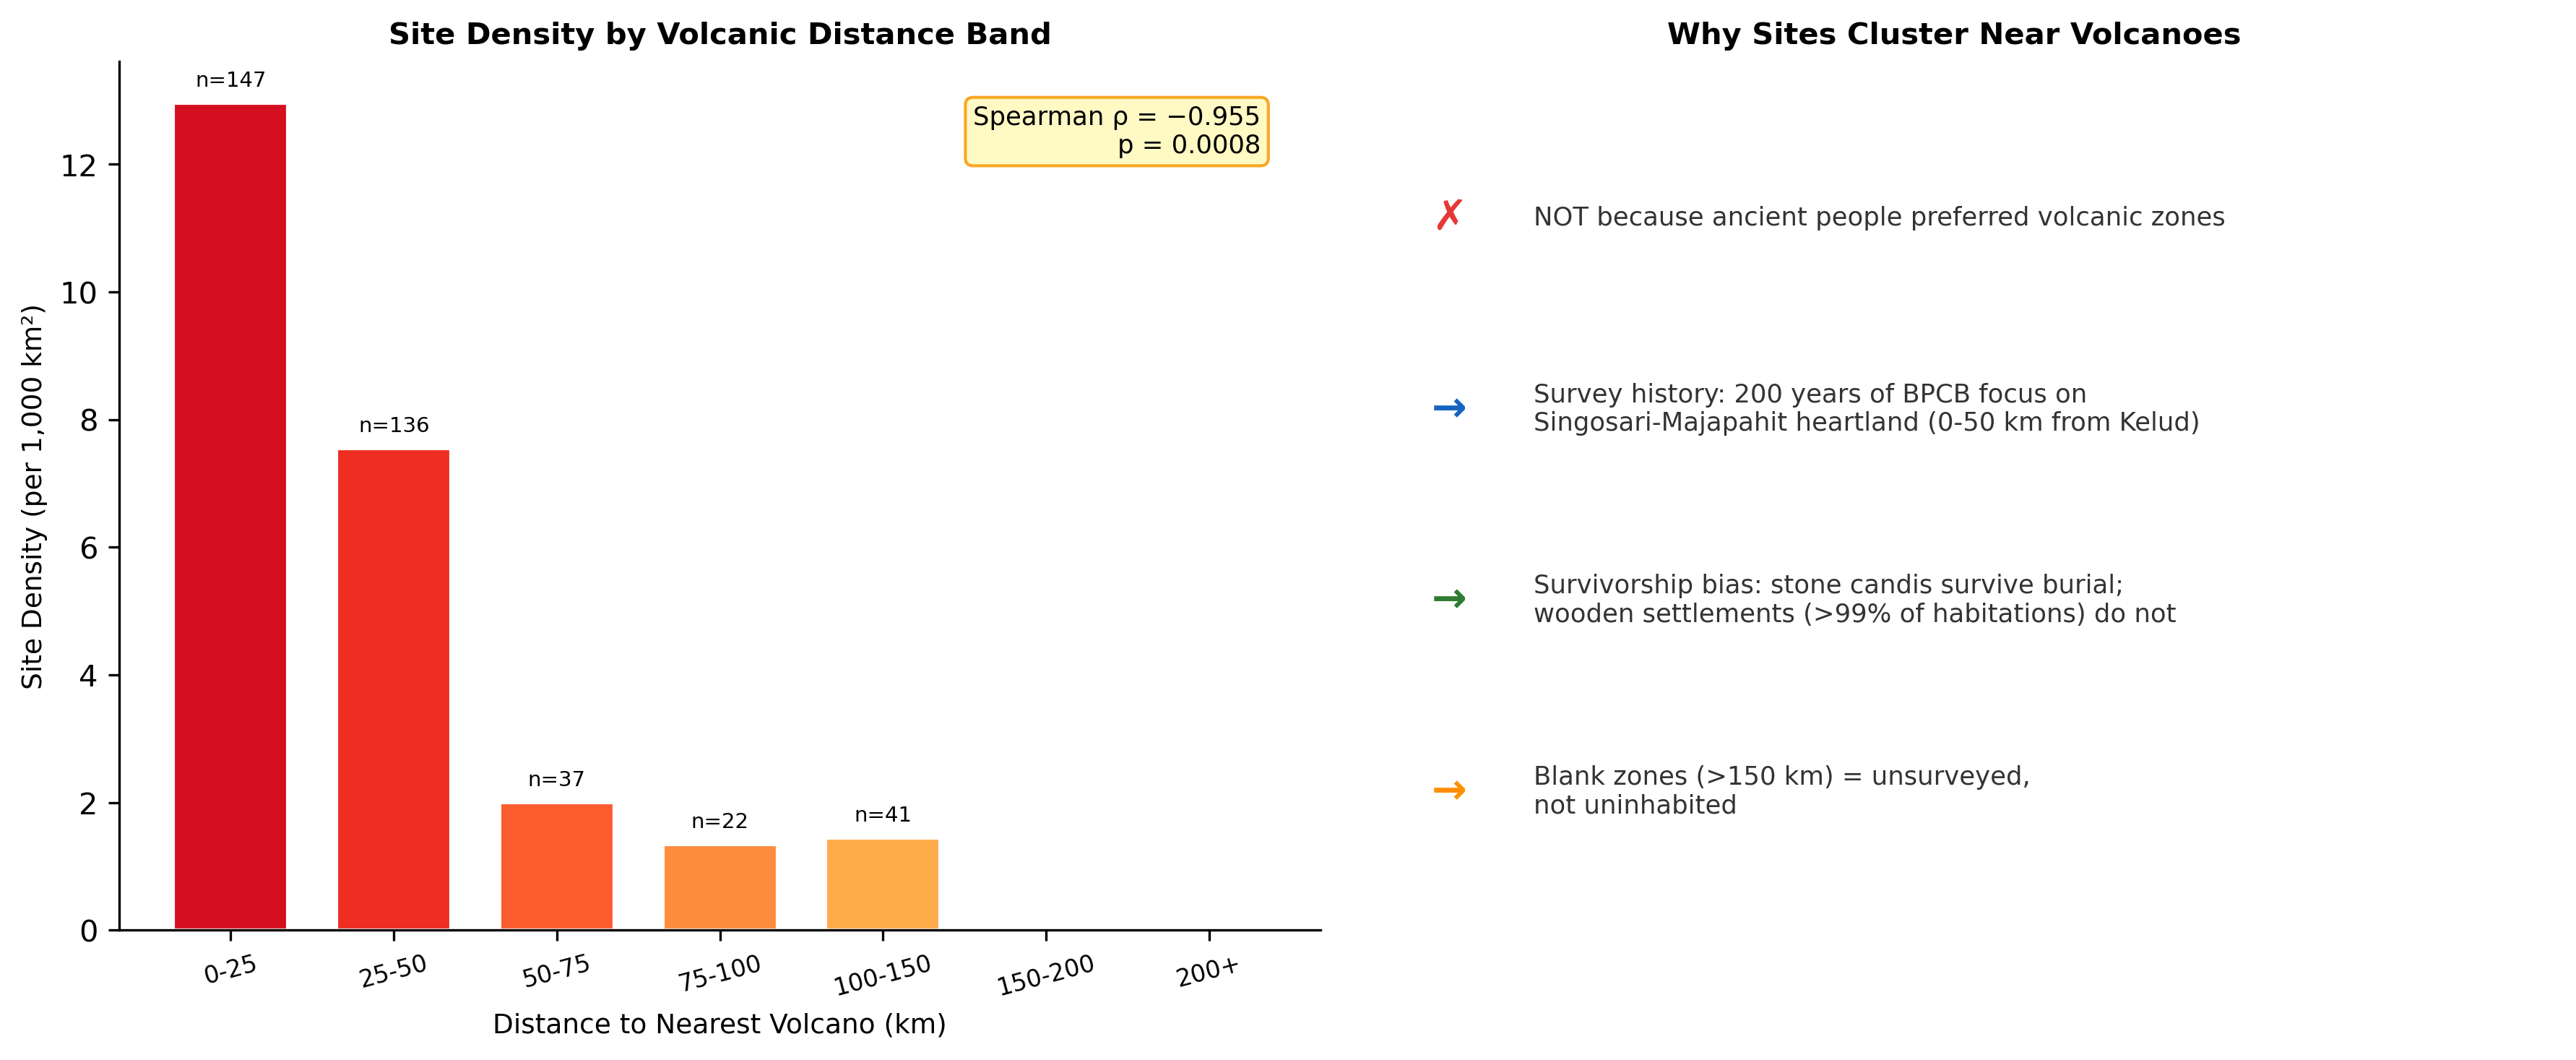
\includegraphics[width=12cm]{figures/fig4_density_vs_distance.png}
\caption{Left: Site density by volcanic distance band showing strong near-volcano clustering ($\rho = -0.955$). Right: Interpretive framework explaining why this pattern reflects survey history, not settlement preference.}
\label{fig:density}
\end{figure*}

The terrain-controlled analysis using a composite terrain suitability index (slope, elevation, TWI, river proximity) across 187 grid cells of 25~km $\times$ 25~km yielded Spearman's $\rho = -0.358$ ($p < 0.0001$). Terrain suitability explains part of the near-volcano clustering, but a substantial residual signal reflects survey intensity concentrated on the Singosari-Majapahit heartland. Repeating both analyses after geocoding 94 additional sites (increasing from 297 to 391 geocoded entries) produced negligible change: the raw density correlation shifted from $-0.991$ to $-0.955$ and the terrain-controlled correlation from $-0.364$ to $-0.358$. The pattern is robust to dataset expansion.

Critically, these results do \textit{not} test the taphonomic bias hypothesis. The fundamental limitation is circular: the sites in this dataset are those that \textit{survived} burial and were \textit{discovered} by archaeologists. Both processes systematically favor low-burial-depth locations. First, stone temples dominate the dataset because they are large enough to protrude through meters of sediment, whereas wooden and bamboo structures---comprising more than 99\% of historical habitation---leave no surface trace after burial (survivorship bias). Second, Indonesian archaeological survey has concentrated on regions of known historical kingdoms for over two centuries, so that ``blank'' areas on the archaeological map are blank because they are unsurveyed, not because they were uninhabited (survey bias). Third, most deeply buried temples were found accidentally during modern construction rather than through systematic survey---Sambisari was exposed by a farmer's plow in 1966, Kimpulan during a university excavation in 2009, and Liangan during sand mining in 2008 \citep{putra2019,abbas2016}---suggesting that the discovery rate is controlled by construction activity rather than archaeological intent (discovery mechanism bias).

The taphonomic bias hypothesis therefore cannot be confirmed or rejected from distribution data alone. It remains a hypothesis requiring subsurface investigation to test. What distribution data \textit{can} establish is the null case: the ``archaeological absence'' of pre-Majapahit evidence in volcanic zones cannot be interpreted as evidence of cultural absence.


\section{Discussion}

\subsection{Significance of the 4.4~mm/yr convergence}

The central empirical result is the convergence of sedimentation rates at $4.4 \pm 1.2$~mm/yr across four sites, two volcanic systems, and 350~km of separation. For a process as variable as volcanic sedimentation---driven by eruption frequency, vent distance, wind direction, and local topography---this degree of agreement across independent systems is noteworthy.

The Kelud-system rate (Dwarapala, 3.5~mm/yr) is lower than the Merapi-system rates (mean approximately 4.8~mm/yr), which is physically reasonable given that Merapi erupts more frequently. Both systems produce the same order-of-magnitude result, indicating that cumulative volcanic burial operates at consistent rates across Java's major volcanic basins.

\subsection{Near-volcano site clustering as a predicted outcome}

The spatial analysis produces a result that appears, at first glance, to refute the taphonomic hypothesis: known sites cluster \textit{near} volcanoes, not away from them ($\rho = -0.955$). However, this pattern is precisely what the taphonomic framework predicts once the composition of the dataset is considered.

The 666 sites in the database are not a random sample of all past settlements. They are the sites that were large enough to protrude through accumulated sediment and that were located in places where archaeologists have concentrated their efforts. The Singosari-Majapahit heartland near Malang and Mojokerto has been surveyed intensively since the Dutch colonial period. This region is also where Kelud and Arjuno-Welirang deposit the most ash. Sites are found there because archaeologists have looked there, and those particular sites survived because they are massive stone monuments. The addition of 94 further geocoded sites from supplementary sources shifted the spatial correlation by only 0.036, suggesting that the database is approaching saturation---not of the actual distribution of past habitation, but of the limits of existing survey coverage.

\subsection{Practical implications for fieldwork}

The burial depth projections translate directly into survey recommendations that differ significantly from standard practice in Indonesian archaeology. Ground-penetrating radar is effective to approximately 2--5~m in volcanic ash \citep{conyers2004}. Late Majapahit-era remains (projected depth 1.5--3.9~m) fall within this detectable range, but Kanjuruhan-era remains (3.0--7.9~m) approach or exceed the practical limits of GPR penetration. Areas with simultaneously high terrain suitability and deep predicted burial represent the highest-priority zones for subsurface investigation, as these are locations where settlement remains are most likely to be preserved yet most likely to remain undetected by surface methods. The pattern of accidental discoveries during modern construction---at Sambisari, Kimpulan, and Liangan---demonstrates that deeply buried sites exist, but systematic subsurface survey targeting such sites has never been conducted in Java.

\subsection{The Kutai comparison}

At 4.4~mm/yr, a Kutai-era (\textasciitilde400~CE) artifact in the Malang basin would now lie beneath approximately 7~m of overburden. The same artifact in Kalimantan, which has no active volcanism, remains at the original ground surface. The perceived chronological primacy of Kutai over Javanese polities of similar antiquity may reflect this differential preservation rather than genuine temporal precedence \citep{coedes1968}.

\subsection{A multiplicative visibility cascade: reframing the primary constraint}

Volcanic burial is not the primary reason that early Javanese sites are invisible; survey coverage is. A five-factor multiplicative visibility model makes this explicit:

\begin{equation}
  P(\text{visible}) = P(\text{not buried}) \times P(\text{organic survival}) \times P(\text{surveyed}) \times P(\text{recognized}) \times P(\text{published})
\end{equation}

We stress that the following are order-of-magnitude estimates, not precise measurements. Volcanic burial survival ($P \approx 0.58$) derives from the four-site calibration; organic material survival ($P \approx 0.20$) from tropical decomposition literature and the observation that 63\% of inscription-mentioned materials are perishable organics; survey coverage ($P \approx 0.025$) from the ratio of systematically surveyed area to total habitable land; recognition probability ($P \approx 0.40$) and publication probability ($P \approx 0.50$) from professional judgment informed by the colonial-era reporting record. Each factor carries substantial uncertainty, but their product---0.058\% predicted visibility---falls within a factor of two of the observed rate (0.031\%, based on 3 ambiguous pre-400~CE sites against approximately 9,600 settlements expected from demographic modeling). The agreement may be partly fortuitous, but the framework identifies which factors contribute most to the overall invisibility.

Survey coverage emerges as the dominant bottleneck: improving it alone would multiply the number of observable sites by approximately 40-fold. Volcanic burial contributes a leverage ratio of only 1.7-fold---the smallest of the five factors. However, volcanic burial is the \textit{only} factor that is spatially predictable. It is not possible to map where organic materials have decayed, where survey effort has been insufficient, or where pre-Hindu sites were misidentified by colonial-era researchers. It \textit{is} possible to map where volcanic burial is deepest. This is the practical value of the calibration framework: not that burial explains everything, but that it provides spatially explicit predictions about where to look.

A separate regression analysis corroborates this conclusion from a different angle. After controlling for three independent survey intensity proxies---road accessibility, distance to BPCB heritage conservation offices, and distance to university archaeology departments---volcanic proximity remained a significant negative predictor of site density (quasi-Poisson likelihood ratio test: $\beta = -0.477$, $p = 0.0015$, correcting for overdispersion $\phi = 3.55$, $n = 703$ grid cells). The volcanic site deficit is not reducible to differential survey effort; a residual burial signal persists after accounting for survey intensity.

A note on what this paper does not claim: one might expect volcanic burial to leave a signature in site-type distributions, selectively destroying open-air sites while leaving caves and rockshelters unaffected. Comparative analysis of 80 Island Southeast Asian sites across volcanic and non-volcanic regions finds no such difference (Fisher exact $p = 0.760$). Cave dominance in the archaeological record is driven by karst availability, not volcanic burial. The taphonomic framework presented here rests entirely on burial depth measurements: 32 burial-depth measurements compiled from Dutch colonial-era excavation reports \citep{ov1925}, averaging 2.88~m, a sedimentation model validated at $r = 0.951$ against observed depths, and the 51-pair eruption--site correlation dataset. The depth-based argument is strengthened, not weakened, by the absence of a site-type effect.

\subsection{Limitations}

The calibration sample of four sites, while spanning two volcanic systems and 350~km of Java, remains small. Rates carry uncertainty from imprecise construction dates and variable depth measurements across sources (e.g., Sambisari depths range from ``5~m'' to ``6.5~m'' depending on the source). All four primary calibration points are stone monuments rather than open habitation sites, and vertical structures may trap sediment preferentially. However, the independent eruption--site correlation dataset---51 pairs across 12 volcanic systems, including non-monumental contexts---yields a mean burial depth of 3.41~m, consistent with the four-point calibration, suggesting that monument-derived and settlement-derived rates are comparable at multi-century timescales.

The sedimentation model treats burial as temporally uniform, smoothing over episodic large eruptions. This is a deliberate modeling choice: the Dwarapala rate averages over approximately 535 years, and the Merapi-system rates average over 1,100--1,200 years. Multi-century averaging inherently incorporates multiple eruptive cycles of varying intensity, and the wide projection range (2.4--6.2~mm/yr) partially captures inter-site variability. Nevertheless, rates derive from only two volcanic basins, and extrapolation to other regions of Java requires additional calibration. Finally, while we argue that survey history dominates distribution data, this claim cannot be quantified precisely without systematic coverage maps, which do not exist for Indonesian archaeological survey.

\subsection{Future directions}

The practical value of the calibration framework depends on its ability to direct fieldwork. The logical next step is a machine learning settlement suitability model that identifies, independently of the burial depth framework, which areas of East Java would have been most attractive to pre-Hindu settlement (Amien, in preparation). Overlaying high suitability with deep predicted burial produces a prioritized list of target zones---locations where evidence is most likely to exist and least likely to have been found. The buried sites at Sambisari and Kimpulan were found by accident; the framework presented here provides a basis for finding the next ones deliberately, through targeted GPR survey and deep coring programs.


\section{Conclusions}

Four calibration points across two volcanic systems and 350~km of separation yield sedimentation rates that converge at 2.4--6.2~mm/yr, with a mean of $4.4 \pm 1.2$~mm/yr. This is a small sample, and we are cautious about generalizing beyond the Kelud and Merapi basins. However, the consistency across geologically distinct volcanic settings suggests that cumulative burial operates at a regional scale, not as a site-specific anomaly.

The implications for archaeological visibility are direct. Kanjuruhan-era remains (\textasciitilde760~CE) in the Malang basin now lie at 3.0--7.9~m depth; pre-Hindu remains (\textasciitilde400~CE) at 3.9--10.1~m. Both ranges exceed conventional surface survey capability and approach the upper limit of ground-penetrating radar. These projections do not prove that early Javanese settlements exist at these depths, but they establish that no systematic search has been conducted where such remains would be located.

The spatial analysis provides an additional constraint. The East Java archaeological record does not map where people lived; it maps where archaeologists have worked and what survived burial by virtue of monumental scale. Stone temples protrude through volcanic sediment because they weigh thousands of tonnes; wooden settlements do not. The concentration of known sites around the Majapahit--Singosari heartland is an artifact of survey history, not evidence of cultural absence from volcanic zones.

The oldest conventionally recognized Indonesian kingdom, Kutai, was found at the modern ground surface in Kalimantan, a region with no active volcanoes. Whether this reflects a coincidence or a consequence of differential preservation is a question that warrants systematic subsurface investigation rather than continued reliance on surface survey alone.


\section*{Data availability}

The archaeological site dataset, DEM derivatives, and analysis scripts are available at \url{https://github.com/neimasilk/volcarch-repo} (to be made public upon acceptance). Raw DEM data from Copernicus GLO-30 are publicly available. A preprint of this manuscript is available at \url{https://doi.org/10.5281/zenodo.19081502}.


\section*{Author contributions}

Conceptualization, M.A.; methodology, M.A. and G.F.G.; software, M.A. and G.F.G.; validation, M.A.; formal analysis, M.A.; investigation, M.A.; data curation, M.A.; writing---original draft, M.A.; writing---review and editing, M.A. and G.F.G.; visualization, M.A.

\section*{Competing interests}

The authors declare no competing interests.

\section*{Acknowledgements}

The authors thank the Global Volcanism Program (Smithsonian Institution) for open eruption data, and the OpenStreetMap and Wikidata communities for structured geospatial data.

\textit{AI assistance disclosure.} This research used AI language tools (Claude, Anthropic) for three tasks: systematic screening of historical, epigraphic, and volcanological literature; iterative design and execution of computational experiments; and manuscript drafting and revision. Research design, hypothesis formation, data selection, interpretation, and all conclusions are solely the authors' intellectual contribution. The authors take full responsibility for all claims made in this paper.


\bibliographystyle{apalike}
\bibliography{references}

\end{document}
